\documentclass[11pt,a4paper,oneside]{report}             % Single-side
%\documentclass[11pt,a4paper,twoside,openright]{report}  % Duplex

%\PassOptionsToPackage{chapternumber=Huordinal}{magyar.ldf}
\usepackage[T1]{fontenc}
\usepackage[utf8]{inputenc}
\usepackage{amsmath}
\usepackage{amssymb}
\usepackage{enumerate}
\usepackage[thmmarks]{ntheorem}
\usepackage{graphics}
\usepackage{epsfig}
%\usepackage{listings}
\usepackage{listingsutf8} % Ezzel a csomaggal működik rendesen a listings UTF-8 esetén is.
\usepackage{color}
%\usepackage{fancyhdr}
\usepackage{lastpage}
\usepackage{anysize}
\usepackage[magyar]{babel}
\usepackage{sectsty}
\usepackage{setspace}  % Ettol a tablazatok, abrak, labjegyzetek maradnak 1-es sorkozzel!
\usepackage[hang]{caption}
\usepackage{hyperref}

% Táblázatoknak:
\usepackage{colortbl}

\usepackage{verbatim}

%--------------------------------------------------------------------------------------
% Main variables
%--------------------------------------------------------------------------------------
\newcommand{\vikszerzo}{Nádudvari György}
\newcommand{\vikkonzulens}{Huszerl Gábor}
\newcommand{\vikcim}{Oktatás támogató rendszerek kiszolgáló infrastruktúrájának felügyeleti lehetőségei}
\newcommand{\viktanszek}{Méréstechnika és Információs Rendszerek Tanszék}
\newcommand{\vikdoktipus}{Szakdolgozat}

%--------------------------------------------------------------------------------------
% Page layout setup
%--------------------------------------------------------------------------------------
% we need to redefine the pagestyle plain
% another possibility is to use the body of this command without \fancypagestyle
% and use \pagestyle{fancy} but in that case the special pages
% (like the ToC, the References, and the Chapter pages)remain in plane style

\pagestyle{plain}
%\setlength{\parindent}{0pt} % áttekinthetőbb, angol nyelvű dokumentumokban jellemző
%\setlength{\parskip}{8pt plus 3pt minus 3pt} % áttekinthetőbb, angol nyelvű dokumentumokban jellemző
\setlength{\parindent}{12pt} % magyar nyelvű dokumentumokban jellemző
\setlength{\parskip}{0pt}    % magyar nyelvű dokumentumokban jellemző

\marginsize{35mm}{25mm}{15mm}{15mm} % anysize package
\setcounter{secnumdepth}{0}
\sectionfont{\large\upshape\bfseries}
\setcounter{secnumdepth}{2}
\singlespacing
\frenchspacing

%--------------------------------------------------------------------------------------
%	Setup hyperref package
%--------------------------------------------------------------------------------------
\hypersetup{
    bookmarks=true,            % show bookmarks bar?
    unicode=false,             % non-Latin characters in Acrobat’s bookmarks
    pdftitle={\vikcim},        % title
    pdfauthor={\vikszerzo},    % author
    pdfsubject={\vikdoktipus}, % subject of the document
    pdfcreator={\vikszerzo},   % creator of the document
    pdfproducer={Producer},    % producer of the document
    pdfkeywords={keywords},    % list of keywords
    pdfnewwindow=true,         % links in new window
    colorlinks=true,           % false: boxed links; true: colored links
    linkcolor=black,           % color of internal links
    citecolor=black,           % color of links to bibliography
    filecolor=black,           % color of file links
    urlcolor=black             % color of external links
}

%--------------------------------------------------------------------------------------
% Set up listings
%--------------------------------------------------------------------------------------
\lstset{
	basicstyle=\scriptsize\ttfamily, % print whole listing small
	keywordstyle=\color{black}\bfseries\underbar, % underlined bold black keywords
	identifierstyle=, 					% nothing happens
	commentstyle=\color{white}, % white comments
	stringstyle=\scriptsize\sffamily, 			% typewriter type for strings
	showstringspaces=false,     % no special string spaces
	aboveskip=3pt,
	belowskip=3pt,
	columns=fixed,
	backgroundcolor=\color{lightgray},
	extendedchars=\true, % Kiegészítés az UTF-8 támogatáshoz
    inputencoding=utf8,
} 		
\def\lstlistingname{lista}	

%--------------------------------------------------------------------------------------
%	Some new commands and declarations
%--------------------------------------------------------------------------------------
\newcommand{\code}[1]{{\upshape\ttfamily\scriptsize\indent #1}}

% define references
\newcommand{\figref}[1]{\ref{fig:#1}.}
\renewcommand{\eqref}[1]{(\ref{eq:#1})}
\newcommand{\listref}[1]{\ref{listing:#1}.}
\newcommand{\sectref}[1]{\ref{sect:#1}}
\newcommand{\tabref}[1]{\ref{tab:#1}.}

\DeclareMathOperator*{\argmax}{arg\,max}
%\DeclareMathOperator*[1]{\floor}{arg\,max}
\DeclareMathOperator{\sign}{sgn}
\DeclareMathOperator{\rot}{rot}
\definecolor{lightgray}{rgb}{0.95,0.95,0.95}

\author{\vikszerzo}
\title{\viktitle}

\begin{comment}
\includeonly{
	guideline,%
	project,%
	titlepage,%
	declaration,%
	abstract,%
	introduction,%
	fejezet_lmsek,
	fejezet_lmsek_it_struk,
	acknowledgement,%
	appendices,%
}
\end{comment}
%--------------------------------------------------------------------------------------
%	Setup captions
%--------------------------------------------------------------------------------------
\captionsetup[figure]{
%labelsep=none,
%font={footnotesize,it},
%justification=justified,
width=.75\textwidth,
aboveskip=10pt}

\renewcommand{\captionlabelfont}{\small\bf}
\renewcommand{\captionfont}{\footnotesize\it}

%###########################################
% Saját eszközök:
%
\definecolor{todobgszin}{rgb}{0.64,0.78,0.22}
\definecolor{todofrszin}{rgb}{0.00,0.50,0.00}
\newcommand{\todo}[1]{\fcolorbox{todofrszin}{todobgszin}{\emph{TODO: #1 }}}


%--------------------------------------------------------------------------------------
% Table of contents and the main text
%--------------------------------------------------------------------------------------
\begin{document}
\singlespacing
%--------------------------------------------------------------------------------------
% Rovid formai es tartalmi tajekoztato
%--------------------------------------------------------------------------------------

\footnotesize
\begin{center}
\large
\textbf{\Large �ltal�nos inform�ci�k, a diplomaterv szerkezete}\\
\end{center}

A diplomaterv szerkezete a BME Villamosm�rn�ki �s Informatikai Kar�n:
\begin{enumerate}
\item	Diplomaterv feladatki�r�s
\item	C�moldal
\item	Tartalomjegyz�k
\item	A diplomatervez� nyilatkozata az �n�ll� munk�r�l �s az elektronikus adatok kezel�s�r�l
\item	Tartalmi �sszefoglal� magyarul �s angolul
\item	Bevezet�s: a feladat �rtelmez�se, a tervez�s c�lja, a feladat indokolts�ga, a diplomaterv fel�p�t�s�nek r�vid �sszefoglal�sa
\item	A feladatki�r�s pontos�t�sa �s r�szletes elemz�se
\item	El�zm�nyek (irodalomkutat�s, hasonl� alkot�sok), az ezekb�l levonhat� k�vetkeztet�sek
\item	A tervez�s r�szletes le�r�sa, a d�nt�si lehet�s�gek �rt�kel�se �s a v�lasztott megold�sok indokl�sa
\item	A megtervezett m�szaki alkot�s �rt�kel�se, kritikai elemz�se, tov�bbfejleszt�si lehet�s�gek
\item	Esetleges k�sz�netnyilv�n�t�sok
\item	R�szletes �s pontos irodalomjegyz�k
\item	F�ggel�k(ek)
\end{enumerate}

Felhaszn�lhat� a k�vetkez� oldalt�l kezd�d� \LaTeX-Diplomaterv sablon dokumentum tartalma. 

A diplomaterv szabv�nyos m�ret� A4-es lapokra ker�lj�n. Az oldalak t�k�rmarg�val k�sz�ljenek (mindenhol 2.5cm, baloldalon 1cm-es k�t�ssel). Az alap�rtelmezett bet�k�szlet a 12 pontos Times New Roman, m�sfeles sork�zzel.

Minden oldalon - az els� n�gy szerkezeti elem kiv�tel�vel - szerepelnie kell az oldalsz�mnak.

A fejezeteket decim�lis beoszt�ssal kell ell�tni. Az �br�kat a megfelel� helyre be kell illeszteni, fejezetenk�nt decim�lis sz�mmal �s kifejez� c�mmel kell ell�tni. A fejezeteket decim�lis al�oszt�ssal sz�mozzuk, maxim�lisan 3 al�oszt�s m�lys�gben (pl. 2.3.4.1.). Az �br�kat, t�bl�zatokat �s k�pleteket c�lszer� fejezetenk�nt k�l�n sz�mozni (pl. 2.4. �bra, 4.2 t�bl�zat vagy k�pletn�l (3.2)). A fejezetc�meket igaz�tsuk balra, a norm�l sz�vegn�l viszont haszn�ljunk sorkiegyenl�t�st. Az �br�kat, t�bl�zatokat �s a hozz�juk tartoz� c�met igaz�tsuk k�z�pre. A c�m a jel�lt r�sz alatt helyezkedjen el.

A k�peket lehet�leg rajzol� programmal k�sz�ts�k el, az egyenleteket egyenlet-szerkeszt� seg�ts�g�vel �rj�k le (A \LaTeX~ehhez k�zenfekv� megold�sokat ny�jt).

Az irodalomjegyz�k sz�vegk�zi hivatkoz�sa t�rt�nhet a Harvard-rendszerben (a szerz� �s az �vsz�m megad�s�val) vagy sorsz�mozva. A teljes lista n�vsor szerinti sorrendben a sz�veg v�g�n szerepeljen (sorsz�mozott irodalmi hivatkoz�sok eset�n hivatkoz�si sorrendben). A szakirodalmi forr�sok c�meit azonban mindig az eredeti nyelven kell megadni, esetleg z�r�jelben a ford�t�ssal. A list�ban szerepl� valamennyi publik�ci�ra hivatkozni kell a sz�vegben (a \LaTeX-sablon a Bib\TeX~seg�ts�g�vel mindezt automatikusan kezeli). Minden publik�ci� a szerz�k ut�n a k�vetkez� adatok szerepelnek: foly�irat cikkekn�l a pontos c�m, a foly�irat c�me, �vfolyam, sz�m, oldalsz�m t�l-ig. A foly�irat c�meket csak akkor r�vid�ts�k, ha azok nagyon k�zismertek vagy nagyon hossz�ak. Internet hivatkoz�sok megad�sakor fontos, hogy az el�r�si �t el�tt megadjuk az oldal tulajdonos�t �s tartalm�t (mivel a link egy id� ut�n ak�r el�rhetetlenn� is v�lhat), valamint az el�r�s id�pontj�t.

\vspace{5mm}
Fontos:
\begin{itemize}
	\item A szakdolgozat k�sz�t� / diplomatervez� nyilatkozata (a jelen sablonban szerepl� sz�vegtartalommal) k�telez� el��r�s Karunkon ennek hi�ny�ban a szakdolgozat/diplomaterv nem b�r�lhat� �s nem v�dhet� !
	\item Mind a dolgozat, mind a mell�klet maxim�lisan 15 MB m�ret� lehet !
\end{itemize}

\vspace{5mm}
\begin{center}
J� munk�t, sikeres szakdolgozat k�sz�t�st ill. diplomatervez�st k�v�nunk !
\end{center}

\normalsize

%--------------------------------------------------------------------------------------
% Feladatkiiras (a tanszeken atveheto, kinyomtatott valtozat)
%--------------------------------------------------------------------------------------
\clearpage
\begin{center}
\large
\textbf{FELADATKI�R�S}\\
\end{center}

A feladatki�r�st a tansz�ki adminisztr�ci�ban lehet �tvenni, �s a leadott munk�ba eredeti, tansz�ki pecs�ttel ell�tott �s a tansz�kvezet� �ltal al��rt lapot kell belef�zni (ezen oldal \emph{helyett}, ez az oldal csak �tmutat�s). Az elektronikusan felt�lt�tt dolgozatban m�r nem kell beleszerkeszteni ezt a feladatki�r�st.





\pagenumbering{arabic}
\onehalfspacing
%--------------------------------------------------------------------------------------
%	The title page
%--------------------------------------------------------------------------------------
\begin{titlepage}
\begin{center}

\includegraphics[width=60mm,keepaspectratio]{figures/BMElogo.png}\\
\vspace{0.3cm}
\textbf{Budapesti Műszaki és Gazdaságtudományi Egyetem}\\
\textmd{Villamosmérnöki és Informatikai Kar}\\
\textmd{\viktanszek}\\[5cm]

\vspace{0.4cm}
{\huge \bfseries \vikcim}\\[0.8cm]
\vspace{0.5cm}
\textsc{\Large \vikdoktipus}\\[4cm]

\begin{tabular}{cc}
 \makebox[7cm]{\emph{Készítette}} & \makebox[7cm]{\emph{Konzulens}} \\
 \makebox[7cm]{\vikszerzo} & \makebox[7cm]{\vikkonzulens}
\end{tabular}

\vfill
{\large \today}
\end{center}
\end{titlepage}



\tableofcontents\vfill
%--------------------------------------------------------------------------------------
% Nyilatkozat
%--------------------------------------------------------------------------------------
\begin{center}
\large
\textbf{HALLGATÓI NYILATKOZAT}\\
\end{center}

Alulírott \emph{\vikszerzo}, szigorló hallgató kijelentem, hogy ezt a szakdolgozatot/ diplomatervet \textcolor{blue}{(nem kívánt törlendő)} meg nem engedett segítség nélkül, saját magam készítettem, csak a megadott forrásokat (szakirodalom, eszközök stb.) használtam fel. Minden olyan részt, melyet szó szerint, vagy azonos értelemben, de átfogalmazva más forrásból átvettem, egyértelműen, a forrás megadásával megjelöltem.

Hozzájárulok, hogy a jelen munkám alapadatait (szerző(k), cím, angol és magyar nyelvű tartalmi kivonat, készítés éve, konzulens(ek) neve) a BME VIK nyilvánosan hozzáférhető elektronikus formában, a munka teljes szövegét pedig az egyetem belső hálózatán keresztül (vagy autentikált felhasználók számára) közzétegye. Kijelentem, hogy a benyújtott munka és annak elektronikus verziója megegyezik. Dékáni engedéllyel titkosított diplomatervek esetén a dolgozat szövege csak 3 év eltelte után válik hozzáférhetővé.

\begin{flushleft}
\vspace*{1cm}
Budapest, \today
\end{flushleft}

\begin{flushright}
 \vspace*{1cm}
 \makebox[7cm]{\rule{6cm}{.4pt}}\\
 \makebox[7cm]{\emph{\vikszerzo}}\\
 \makebox[7cm]{hallgató}
\end{flushright}
\thispagestyle{empty}

\vfill
\clearpage
\thispagestyle{empty} % an empty page


%----------------------------------------------------------------------------
% Abstract in hungarian
%----------------------------------------------------------------------------
\chapter*{Kivonat}\addcontentsline{toc}{chapter}{Kivonat}

Jelen dokumentum egy diplomaterv sablon, amely formai keretet ad a BME Villamosmérnöki és Informatikai Karán végző hallgatók által elkészítendő szakdolgozatnak és diplomatervnek. A sablon használata opcionális. Ez a sablon \LaTeX~alapú, a \emph{TeXLive} \TeX-implementációval és a PDF-\LaTeX~fordítóval működőképes.
\vfill

%----------------------------------------------------------------------------
% Abstract in english
%----------------------------------------------------------------------------
\chapter*{Abstract}\addcontentsline{toc}{chapter}{Abstract}

This document is a \LaTeX-based skeleton for BSc/MSc~theses of students at the Electrical Engineering and Informatics Faculty, Budapest University of Technology and Economics. The usage of this skeleton is optional. It has been tested with the \emph{TeXLive} \TeX~implementation, and it requires the PDF-\LaTeX~compiler.
\vfill


%----------------------------------------------------------------------------
\chapter*{Bevezet�}\addcontentsline{toc}{chapter}{Bevezet�}
%----------------------------------------------------------------------------

A bevezet� tartalmazza a diplomaterv-ki�r�s elemz�s�t, t�rt�nelmi el�zm�nyeit, a feladat indokolts�g�t (a motiv�ci� le�r�s�t), az eddigi megold�sokat, �s ennek t�kr�ben a hallgat� megold�s�nak �sszefoglal�s�t.

A bevezet� szok�s szerint a diplomaterv fel�p�t�s�vel z�r�dik, azaz annak r�vid le�r�s�val, hogy melyik fejezet mivel foglalkozik.


\chapter{Tanulásmenedzsment rendszerek}
Tanulásmenedzsment rendszernek, angolul Learning Management Systemnek (LMS-nek) nevezzük azokat a szoftver alkalmazásokat, amelyek automatizálják az oktatás adminisztrációját, követését, az online kurzusok és az azokkal kapcsolatos események, anyagok kezelését.

Egy robusztus LMS-nek képesnek kell lennie \cite{link:ell}:
\begin{itemize}
\setlength{\itemsep}{0pt}
\item központosított és automatizált adminisztrációra,
\item önkiszolgáló és önálló irányítású szolgáltatások nyújtására,
\item oktatási anyagok gyors összeállítására és elérhetőségének biztosítására,
\item konszolidált képzési kezdeményezésekre skálázható, web alapú platformon,
\item a portabilitás és a szabványok támogatására,
\item személyre szabott tartalom előállítására és a tudás újrafelhasználásának lehetővé tételére.
\end{itemize}

Tehát egy tanulásmenedzsment rendszer nem más, mint olyan szolgáltatások összessége, amelyek támogatják a rendszer felhasználóinak adminisztrálását, jogosultságok kiosztását, új tartalmak, oktatási anyagok létrehozását, elérhetővé tételét, megosztását, a felhasználók tanulmányi menetének követését, irányítását, felkészültségüknek ellenőrzését, általában webes platformon, más rendszerekkel szabványosan együtt működve. Az LMS-ek általában lehetőséget biztosítanak, arra is, hogy a felhasználók a rendszeren keresztül kommunikáljanak is egymással.

Fontos megjegyezni, hogy nem csak a közoktatásban, hanem a vállalati, ipari továbbképzésekben is szívesen alkalmazzák ezeket a rendszerek, mivel sok közülük rendelkezik a megfelelő humánerőforrás kezeléssel kapcsolatos funkciókkal is.

A piacon több nyílt forrású, ingyenesen elérhető és zárt, kereskedelmi változatokat, vagy vegyes koncepciókat is találunk, amelyek esetében ugyan a rendszer maga nyílt forrású, de a támogatásért, vagy akár bérüzemeltetésért már pénzbeli juttatást kérnek. \Aref{tab:openlms}.~táblázatban néhány ismertebb nyílt forrású LMS-t soroltam fel \cite{link:lms}. Érdemes megnézni, hogy általában PHP, MySQL technológiák segítségével valósítják meg ezeket a rendszereket.

\definecolor{MyTableColor}{rgb}{0.38,0.28,0.25} 

\begin{table}[h]
	\caption{Néhány elterjedtebb LMS}
	\centering
	\small
	\begin{tabular}{| p{1.6cm} | p{4.4cm} | p{2.2cm} | p{3.8cm} |}
		\hline
		\rowcolor{MyTableColor} \textbf{Név} & \textbf{Projekt oldal} & \textbf{Használt prog.~nyelv} & \textbf{Támogatott adatbázisok} \\
		\hline
		Sakai & \href{http://www.sakaiproject.org/}{http://www.sakaiproject.org/} & Java & MySQL,~Oracle,~DB2 \\
		\hline
		Moodle & \href{http://moodle.org/}{http://moodle.org/} & PHP & MySQL, PostgreSQL, MSSQL, Oracle \\
		\hline
		OLAT &  \href{http://www.olat.org/}{http://www.olat.org/} & Java & MySQL,~PostgreSQL \\
		\hline
		Instructure - Canvas & \href{http://www.instructure.com/}{http://www.instructure.com/} & Ruby on Rails & PostgreSQL \\
		\hline
		ILIAS & \href{http://www.ilias.de/docu/}{http://www.ilias.de/docu/} & PHP & MySQL, Oracle 11g \\
		\hline
		Dokeos & \href{http://www.dokeos.com/}{http://www.dokeos.com/} & PHP & MySQL \\
		\hline
		Chamilo & \href{http://www.chamilo.org/}{http://www.chamilo.org/} & PHP & MySQL \\
		\hline		
		Claroline & \href{http://www.claroline.net/}{http://www.claroline.net/} & PHP & MySQL \\
		\hline
	\end{tabular}
	\normalsize
	\label{tab:openlms}
\end{table}


Adott a kérdés, hogy mi lehet ennek az oka? Mivel ezek a legelterjedtebb nyílt forrású technológiák, és teljesítményben is megfelelnek egy LMS-nél megjelenő kérések kiszolgálására

\todo{<- Megfogalmazni} 

Kereskedelmi termékekről nem sikerült érdemleges információhoz jutni az alkalmazott technológiákról, de feltételezhető a Java, .NET platformok használata is. A felhasználói oldalon gyakran találunk Flash alapú megvalósításokat.

A HTML5 technológia terjedésének valószínűsíthető következménye lesz, hogy ezekben a rendszerekben is lecserélésre kerül a Flash-es keretrendszer. A HTML5 lehetőséget biztosít arra, hogy az eddigi megjelenést ne kelljen lecserélni, s ezzel a felhasználónak ne kelljen az új rendszerbe beletanulni, ugyanakkor hasonló felülettel találkozzanak az otthoni számítógépük, netbookjuk, táblagépük, vagy mobiltelefonjuk használata során. Ezek mellett fejlesztési oldalon költségcsökkenésre lehet számítani, mert nem kell a különböző eszközökre külön-külön lefejleszteni ugyanazt a grafikus interfészt, ami a HTML5 szabványosságának köszönhető. Az üzemeltetésre is kevesebb teher jut, hiszen ezen technológia nagy része felhasználói oldalon fut, így nem csökken a rendszer teljesítménye.

\todo{Bibliográfia}

\begin{comment}

% TODO

\bibitem[ell] {link:ell}
	Ellis, Ryann K. {\it A Field Guide to Learning Management Systems}, ASTD Learning Circuits, 2009 \\ \href{http://www.astd.org/NR/rdonlyres/12ECDB99-3B91-403E-9B15-7E597444645D/23395/LMS\_fieldguide\_20091.pdf}{http://www.astd.org/NR/rdonlyres/.../LMS\_fieldguide\_20091.pdf}

\bibitem[lms] {link:lms}
	Wikipedia, {\it List of learning management systems} \\ \href{http://en.wikipedia.org/wiki/List\_of\_learning\_management\_systems}{http://en.wikipedia.org/wiki/List\_of\_learning\_management\_systems}

\end{comment}

\chapter{Tanulásmenedzsment rendszerek IT infrastruktúrája}

Ebben a fejezetben a háromrétegű architektúra példáján alapulva részletezem az oktatástámogató rendszerek IT infrastruktúráját, majd egy megvalósítást részletesebben is bemutatok. 

\section{A háromrétegű architektúra}
A webes LSM-ek általában a háromrétegű architektúrát követik. Ez a három réteg a webkiszolgáló, az adatbázis és az alkalmazás réteg. A réteges szerkezetnek köszönhetően ezek a rendszerek jól skálázhatóak, gyakran az egyes rétegekben a réteget megvalósító alkalmazások olyan tulajdonságokkal, funkciókkal rendelkeznek, amelyek támogatják is a skálázás egyszerű, esetleg automatikus megvalósítását.

\begin{figure}[!ht]
\centering
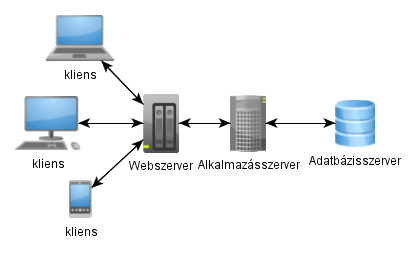
\includegraphics[width=100mm, keepaspectratio]{figures/3tier_simple_001.png}
\caption{A háromrétegű architektúra.}
\label{fig:3tier_simple_001}
\end{figure}

\Aref{fig:3tier_simple_001}.~ábrán látható elrendezéssel ellentétben a rétegeknek nem szükséges fizikailag is külön hardverre kerülni (sőt az alkalmazás- és webkiszolgáló-réteg esetében ez nem is mindig lehetséges), így a legegyszerűbb kialakítás akár egy számítógépet is igénybe vehet. Ez a megoldás egy viszonylag erős konfiguráció és alacsony felhasználószám esetén működhet.

\subsection{A webkiszolgáló réteg}
A webkiszolgáló réteg feladatát egy szolgáltatás látja el, amely futhat egy vagy több példányban, és egy példány futhat egy vagy több számítógépen is. Ez a szolgáltatás felelős azért, hogy a kliensek kérésének megfelelően előálljon a weblap, vagyis a kliensek kérésre kapjanak egy HTML dokumentumot, amelyet a felhasználói oldalon jelenítenek meg.
A piacon több webkiszolgáló alkalmazást találunk, ezek közül van ingyenes, nyílt forráskódú (pl. Apache), és kereskedelmi termék is (Microsoft IIS).

\Aref{fig:netcraft_webservers}.~ábrán a legelterjedtebb webkiszolgálók piaci részesedésének alakulása látható.

\begin{figure}[h!]
\centering
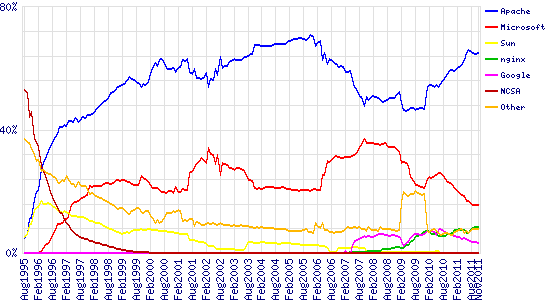
\includegraphics[width=1.0\textwidth]{figures/wpid-overallc.png}
\caption{A legelterjedtebb webszerverek piaci részesedése (2011. november, forrás: \href{http://news.netcraft.com/archives/2011/11/07/november-2011-web-server-survey.html}{Netcraft.com}) \label{fig:netcraft_webservers}}
\end{figure}

Az oktatástámogató rendszerek szempontjából fontos, hogy a működtetett webkiszolgáló képes legyen nagy számú konkurens kérés kiszolgálására, vagy könnyen skálázható, elosztható legyen. LMS-ek esetén is ugyanazokat a webkiszolgálókat lehet használni, mint amit más egyéb webes alkalmazások esetén (pl. Apache, Microsoft IIS, lighttpd, ngnix, stb.).
 
\subsection{Az alkalmazás réteg}
Az alkalmazás réteg feladatát az alkalmazásszerver látja el. Az alkalmazásszerver egy olyan speciális környezet, ahol alkalmazások futhatnak, és amely környezet szempontjából lényegtelen, hogy mik ezek az alkalmazások és mit csinálnak\cite{serverside}. Az alkalmazásszerver eljárások (programok, rutinok, szkriptek) hatékony végrehajtására dedikált erőforrás.

Az első alkalmazásszerverek megjelenésekor fő feladatuk volt, hogy webes alkalmazások esetén a webszerver által megjeleníthető tartalmat állítsanak elő. Ezen továbblépve napjainkban már nem csak az oldalgenerálás funkciója jelenik meg ebben a rétegben, hanem egyéb szolgáltatásokat is implementálnak, mint például klaszterszervezést, terheléselosztást, hibaátállást. Ezen funkciókkal elérhető, hogy az alkalmazásfejlesztőknek csak az üzleti logikával kelljen foglalkozni.

Az LMS-ek lényegi része ebben a rétegben kerül megvalósításra. Mivel a ténylegesen alkalmazott platformtól függ, hogy milyen alkalmazásszervert használunk, ezért alapvetően erről az oldalról nincs megkötés. Ám érdemes figyelembe venni, hogy a kiválasztott platform mennyire skálázható, milyen teljesítményt nyújt a különböző terhelésekre. A legelterjedtebb LMS-ek fejlesztésére használt platformok itt is mint más webes rendszereknél a PHP, Java és .Net.

\subsection{Az adatbázisréteg}
Az adatbázisréteg feladatait az adatbázisszerver látja el. Adatbázisszervernek nevezünk egy dedikált szolgáltatást, ami adatbázisokat tesz elérhetővé, kezelhetővé. Valójában egy felületet biztosít az alkalmazásrétegben található adatfelhasználó alkalmazás és maguk a felhasználandó adatok között.

Az LMS-ek oldaláról igény, hogy a használt adatbázis képes legyen nagy számú konkurens tranzakcióra, és optimálisan tároljon nagy, multimédiás adatokat is. Főleg a költségvetéstől és az üzemeltetéstől függően lehet MySQL, PostgreSQL, Microsoft SQL Server vagy Oracle adatbázisszerver is, de természetesen attól is függ, hogy az adott LMS melyiket támogatja. 

\section{Egy példa: a Moodle rendszer}
Az oktatástámogató rendszerek közül a Moodle rendszerrel részletesebben foglalkoztam. A következő részben bemutatom az általam megismert felépítését, fontosabb jellemzőit, és ejtek néhány szót az általam telepített rendszerről is.

\subsection{A Moodle rendszer felépítése, tulajdonságai}
Az e-learning rendszerek közül a legelterjedtebb a Moodle (Modular Object-Oriented Dynamic Learning Environment) (\href{http://moodle.org}{http://moodle.org}) nevű tanulásmenedzsment rendszer. Korábbi munkám során ennek a rendszernek a részletesebb megismerése volt az egyik cél.

A Moodle  egy ingyenes és nyílt forrású LMS vagy VLE (Virtual Learning Environment, virtuális oktató környezet). 2010 októberében 49952 regisztrált Moodle oldal létezett, amelyek összesen mintegy 37 millió felhasználót szolgáltak ki. A legnagyobb rendszertelepítések közé tartozik a tajvani Ming Chuan Egyetem több mint 63.000 regisztrált, maximálisan 33.000 bejelentkezett felhasználóval naponta \cite{moodleinstplus}.

Maga a rendszer tervezéséből és implementálásából eredően portábilis, hála a PHP nyelvnek. Módosítás nélkül telepíthető Unix, Linux variánsokra, FreeBSD-re, Windows-ra, Mac OS X-re, NetWare-re és egyéb rendszerekre, amelyek támogatják a PHP-t és az ismertebb adatbázis-kezelő rendszereket.

A Moodle architektúrájában elválik a natív adatbázis-kezelő a felsőbb rétegektől. Közöttük egy ADOdb adatbázis absztrakciós réteg található. Az ADOdb egy különálló projekt\footnote{\href{http://adodb.sourceforge.net/}{http://adodb.sourceforge.net/}}, amely a legelterjedtebb adatbázis-kezelőket támogatja. \Aref{fig:moodlearch}.~ábrán egy korábbi verzió architektúrája látható.

\begin{figure}[h!]
\centering
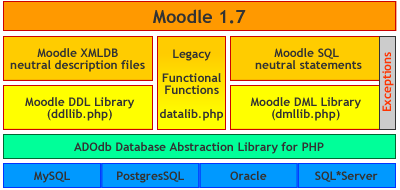
\includegraphics[width=0.65\textwidth]{figures/moodlearch.png}
\caption{A Moodle architektúrája \label{fig:moodlearch}}
\end{figure}

Az architekturális felépítésből látható, hogy a Moodle az ADOdb által nyújtott rétegen keresztül egységesen éri el az eltérő adatbázis-megvalósításokat anélkül, hogy foglalkoznia kellene az ezekből eredő problémákkal.  

Az interoperabilitás több Moodle képességben megjelenik, ilyenek például:
\begin{sajat_itemize}
\setlength{\itemsep}{0pt}
\item autentikáció LDAP-on, Shibboleth-en keresztül
\item kérdések/kérdéssorok importálása/exportálása több formátumban (pl. XML, XHTML stb.)
\item erőforrások kezelése (SCORM, AICC)
\item integráció más tartalomkezelő rendszerekkel (Drupal, Postnuke).
\end{sajat_itemize}

A Moodle fontos tulajdonsága a modularitás, vagyis a rendszer funkcionalitásának könnyű bővíthetősége. Ezt plug-inokkal valósítják meg, amelyek fejlesztését különböző API-k segítik. Ilyen plug-inok pl. a különböző jelentések (reportok), blokkok, portfóliók, tárolók (repository-k), kereső modulok. Ezek közül nagyon sok megtalálható az alap Moodle telepítésben is, de saját magunk is írhatunk hasonló kiegészítőket.

\subsection{Egy lehetséges infrastruktúra kialakítás a Moodle esetében}

Mint azt már említettem, a Moodle nagyon sok operációs rendszerre telepíthető. Én az egyik legelterjedtebb telepítési környezet választottam ki, egy ún. LAMP (Linux - Apache - MySQL - PHP) megoldást használtam. Fizikai szerver helyett virtuális szervert alkalmaztam a Simonyi Károly Szakkollégium Kollégiumi Számítástechnikai Kör erőforrásainak igénybevételével. A virtualizációs megoldás alapja egy VMware ESX szerver volt.
A virtuális szerverem konfigurációja viszonylag gyengének számít, ám nem is volt cél, hogy nagy számú felhasználót szolgáljon ki:
\begin{sajat_itemize}
\item Ubuntu Server 10.10 32bit
\item 512 MB RAM
\item 10 GB tárhely
\item 4 MB RAM a videóvezérlőnek 
\end{sajat_itemize}
Az így kialakított struktúra tulajdonképpen egy egygépes megoldás, mind a webszerver, az alkalmazásszerver, mind az adatbázisszerver egyetlen virtuális gépen futott. Természetesen az infrastruktúra méretét lehetett volna növelni, bonyolítani monitorozó, naplófeldolgozó, biztonsági mentés készítő megoldásokkal, de ez szintén nem volt a feladat része.

\chapter{Tanulásmenedzsment rendszerek erőforrásigényei}
\section{Alapvető igények}
\todo{•}

Minden informatikai rendszernek van erőforrásigénye, vagyis az a minimális hardver konfiguráció, amelyen a rendszer bizonyos számú kéréseket ki tud szolgálni adott időn belül. \todo{Kellene jobb fogalom leírás}
A rendszer erőforrásigénye sok részletből tevődhet össze. 
\todo{Milyen OS-en vagyunk, annak is van alap igénye}
\todo{Webszerverek eltérő igénye}
\todo{Platform igények PHP vs. Java vs. Ruby vs. ASP vs. Python}
\todo{adatbázisok igénye MySQL vs. PostgreSQL vs. Oracle vs. MSSQL}

\subsection{Moodle}
A Moodle hardveres erőforrásigényei a következők:
\begin{itemize}
\item{min. 160 MB tárolókapacitás (csak a rendszernek),}
\item{min. 256 MB memóriakapacitás (1 GB ajánlott).}
\end{itemize}
\todo{CPU}
\todo{I/O}
\todo{Forrás: \href{http://docs.moodle.org/20/en/Installing\_Moodle}}


\section{Igények terhelésváltozások esetén}
\todo{}
\section{Modellek}
\todo{}

%----------------------------------------------------------------------------
\chapter*{Köszönetnyilvánítás}\addcontentsline{toc}{chapter}{Köszönetnyilvánítás}
%----------------------------------------------------------------------------

Ez nem kötelező, akár törölhető is. Ha a szerző szükségét érzi, itt lehet köszönetet nyilvánítani azoknak, akik hozzájárultak munkájukkal ahhoz, hogy a hallgató a szakdolgozatban vagy diplomamunkában leírt feladatokat sikeresen elvégezze. A konzulensnek való köszönetnyilvánítás sem kötelező, a konzulensnek hivatalosan is dolga, hogy a hallgatót konzultálja.

%\listoffigures\addcontentsline{toc}{chapter}{Ábrák jegyzéke}
%\listoftables\addcontentsline{toc}{chapter}{Táblázatok jegyzéke}

\bibliography{mybib}
\addcontentsline{toc}{chapter}{Irodalomjegyzék}
\bibliographystyle{plain}

%----------------------------------------------------------------------------
\appendix
%----------------------------------------------------------------------------
\chapter*{Függelék}\addcontentsline{toc}{chapter}{Függelék}
\setcounter{chapter}{6}  % a fofejezet-szamlalo az angol ABC 6. betuje (F) lesz
\setcounter{equation}{0} % a fofejezet-szamlalo az angol ABC 6. betuje (F) lesz
\numberwithin{equation}{section}
\numberwithin{figure}{section}
\numberwithin{lstlisting}{section}
%\numberwithin{tabular}{section}

%----------------------------------------------------------------------------
\section{Az Amazon AWS néhány fontosabb API metódusa}
%----------------------------------------------------------------------------



\label{page:last}
\end{document}
